%
% File acl2014.tex
%
% Contact: koller@ling.uni-potsdam.de, yusuke@nii.ac.jp
%%
%% Based on the style files for ACL-2013, which were, in turn,
%% Based on the style files for ACL-2012, which were, in turn,
%% based on the style files for ACL-2011, which were, in turn, 
%% based on the style files for ACL-2010, which were, in turn, 
%% based on the style files for ACL-IJCNLP-2009, which were, in turn,
%% based on the style files for EACL-2009 and IJCNLP-2008...

%% Based on the style files for EACL 2006 by 
%%e.agirre@ehu.es or Sergi.Balari@uab.es
%% and that of ACL 08 by Joakim Nivre and Noah Smith

\documentclass[11pt]{article}
\usepackage[utf8]{inputenc}
\usepackage{acl2014}
\usepackage{times}
\usepackage{microtype}
\usepackage{url}
\usepackage{latexsym}
\usepackage{amsmath}
\usepackage{paralist} % inline lists
\usepackage{commands}
\usepackage{cleveref}
\usepackage{placeins} % FloatBarrier

\usepackage{tikz}
\usepackage{pgfplots}

% DEV
\usepackage{booktabs}

% smart quotes
\usepackage[autostyle, english=american]{csquotes}
\MakeOuterQuote{"}

%\setlength\titlebox{5cm}

% You can expand the titlebox if you need extra space
% to show all the authors. Please do not make the titlebox
% smaller than 5cm (the original size); we will check this
% in the camera-ready version and ask you to change it back.


\title{Deep Neural Networks for Bilingual Lexicon Extraction}

%\author{Jon Gauthier\affilA\,and\,Arthur Tsang\affilB \\
%  \affilA Symbolic Systems, \affilB Computer Science \\
%Stanford University, Stanford, CA 94035 \\
%{\tt \{jgauthie,atsang2\}@stanford.edu}}

\date{}

\begin{document}
\maketitle

\begin{abstract}
  We explore a method for producing bilingual lexicons from non-parallel
  corpora. In contrast with most previous approaches, our method separates the steps
  of \begin{inparaenum}[(1)]
    \item constructing distributed word representations from monolingual
      corpora, and
    \item building a mapping between these representations.
  \end{inparaenum}
  This gives us precise control over the independent development of the word representations and the mapping between them.
  %By performing these two steps separately, we gain great flexibility in determining how our word representations are constructed. % are able to construct distributed word representations with greater flexibility. % TODO more specific and contentful
  We demonstrate that a deep neural network can effectively learn a translational
  mapping between these representations for the purposes of bilingual lexicon extraction more accurately than a linear model.
  %explain baseline
  %We suggest that a deep learning model beats a linear baseline by allowing more flexibility. % make this more concrete
\end{abstract}

\section{Introduction}
\label{sec:introduction}

In bilingual lexicon extraction (BLE), we accept as input some pair of corpora
in different languages---perhaps parallel or perhaps not---and use them to learn associations of translational equivalence between a \textit{source language} and a \textit{target language}.

Bilingual lexicon extraction is obviously of most utility when applied to
under-resourced language pairs which do not already benefit from a surplus of
lexicon materials. These same language pairs, lacking resources as simple as quality translation dictionaries, also lack sufficient amounts of manually aligned
text to train BLE models. % briefly mention that each individual language may have a significant corpus though?
For this reason, most recent work on this task focuses on
minimally supervised approaches which do not require parallel corpora
\cite{rapp1995,peirsman2010}.

\newcite{rapp1995} suggested that there is "a correlation between the patterns
of word co-occurrences in different languages." In line with this hypothesis,
recent work has related the likelihood of two words being translations of one
another to the similarities between the contexts in which the words appear in
their corresponding languages. The standard approach under this theory is to
manually construct a \textit{bilingual vector space} which contains distributed
representations of words in both the source and target language
\cite{fung1998,vulic2013}. The axes of this space are built from
bilingual seed pairs. A given word representation has a large value along an axis
if it co-occurs often with the seed word corresponding to that axis. Because
axes are defined with bilingual pairs, word representations for both source and
target language words can lie in the same space. With a bilingual vector space
constructed, translations for a given source-language word can be retrieved by
simply finding the nearest target-language word representation neighboring the
word's own vector representation in the bilingual vector space.

The present paper is motivated by the hypothesis that this standard bilingual
vector space approach to BLE is inherently limited by the design of the space
itself.
% SHORT We suggest that the construction of the space along axes composed of a hand-picked set of bilingual seeds has the potential to limit the expressiveness of the word representations contained therein.
Consider, for example, a vector
space constructed in this fashion using just two seeds: \textit{hot} and
\textit{cold}. Such a space may be effective at representing the difference
between words like \textit{fire} and \textit{ice}. However, with these two axes
it would fail to capture many other distinctions, such as the difference between
the words \textit{up} and \textit{down}. The quality of the vector space is
thus heavily dependent on the quality of its seeds.

\newcite{mikolov2013exploiting} suggest an alternate method for bilingual lexicon
extraction, centered around two monolingual vector spaces $E$ (corresponding to the
source language) and $F$ (corresponding to the target language). These vector spaces
are constructed using a standard neural language model \cite{mikolov2013}. We see this as a promising alternative to the aforementioned bilingual vector space approach, as it allows for the construction of robust distributed representations whose quality is not dependent on manually selected seeds. The authors find
that a linear model trained via stochastic gradient descent to map between these two
vector spaces can effectively map source-language word representations to the
target-language word vectors corresponding to their translations.

We extend this work in attempting to model a \emph{translation function} $t : E \to F$.
% SHORT
% We capitalize on the fact that these vector spaces may be independently constructed, experimenting with different configurations for each space.
In this paper we approximate the transformation $t$ between the two spaces using a deep neural
network, trained to accept as input word vectors from the source language space
$E$ and output word vectors in the target language space $F$.

% \Cref{sec:data} describes the corpora used to test this translation process.
% \Cref{sec:model} details the actual process of translation. In
% \Cref{sec:evaluation,sec:conclusion} we analyze the performance of our model and
% examine how it supports our motivating hypothesis.

\section{Data}
\label{sec:data}

Our translation algorithm makes use of two monolingual corpora: one consisting of text
in the source language and the other containing text in the target language. We presume
the corpora have the following properties:
\subparagraph{Large and broad-domain.} With this property given, we can safely assume
that for any common
word which appears in the source-language corpus, we will also find its
translation somewhere in the target-language corpus.
If large corpora are unavailable, we can make use of smaller narrow-domain corpora, such as religious texts.
\subparagraph{Non-parallel.} This means that our algorithm does not depend on any sort
of alignment, lexical or topical. This relative flexibility allows us to demonstrate
that the method can be applied in situations where parallel corpora are not available.

% TODO for long paper: describe preprocessing techniques (stolen from Gensim).
In our experiments we use English and Spanish corpora sourced from Wikipedia.%
\footnote{Available at \url{http://dumps.wikimedia.org/}.}
We choose not to take advantage of the document alignments available in the Wikipedia corpus in order to show that our method is generalizable to other corpora.

In addition to the two monolingual corpora, we train on a minimal
%, manually-created
set of word translation pairs.
% TODO I don't like "such as a swadesh list" --- Jon
The specifics of these training pairs are described in \Cref{subsec:translation-nn}.

%In addition to using the corpora, we also rely on a small seed set of several hundred English % -Spanish word pairs to train the translation function.
% Include the seed sets as an appendix?

\section{Model}
\label{sec:model}

\begin{figure}[tb!]
	\centering
	\resizebox{\linewidth}{!}{
    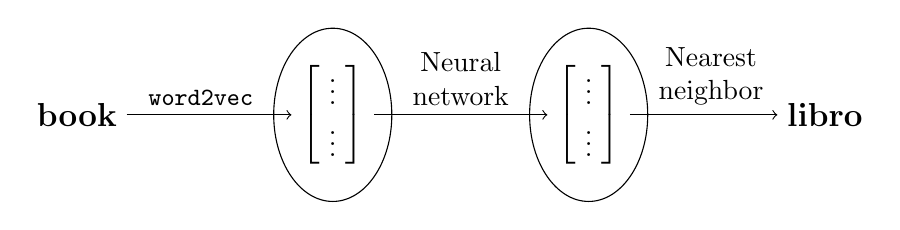
\begin{tikzpicture}
        \node (english) at (0, 2) {\large \textbf{book}};
    
        \draw (3.25, 2) ellipse[x radius=0.75, y radius=1.1];
        \node (englishvec) at (3.25, 2) {$\begin{bmatrix}~\vdots~\\\vdots\end{bmatrix}$};

        \draw (6.5, 2) ellipse[x radius=0.75, y radius=1.1];
        \node (spanishvec) at (6.5, 2) {$\begin{bmatrix}~\vdots~\\\vdots\end{bmatrix}$};

        \node (spanish) at (9.5, 2) {\large \textbf{libro}};

        \draw [->] (english) -- (englishvec) node [pos=0.45, above] {\small \texttt{word2vec}};
        \draw [->] (englishvec) -- (spanishvec) node [midway, above, align=center] {Neural\\network};
        \draw [->] (spanishvec) -- (spanish) node [pos=0.55, above, align=center] {Nearest\\neighbor};
    \end{tikzpicture}
    }
    \caption{The process of word translation, using a neural network to map between
        two monolingual VSMs}
    \label{fig:translation}
\end{figure}

\Cref{fig:translation} illustrates the process of translating a single word from a source
language to a target language (here English and Spanish, respectively) in this model. We
begin with an input source-language word and retrieve a corresponding pre-computed word
representation in the source VSM. We use this source-language word vector as an input to
a neural network, which outputs a vector in the target-language VSM. We perform a simple
nearest-neighbor search in the target-language VSM to find the closest existing word
vector, and take its corresponding target-language word to be the translation of the
original source-language word.

\subsection{Word representations}
\label{subsec:word-representations}

For each of the two corpora introduced in \Cref{sec:data}, we train a continuous vector space model on 10-word contexts, using an implementation in the \textit{Gensim} software package of \texttt{word2vec}, a neural language model \cite{rehurek2010,mikolov2013}. This neural language model attempts to learn word representations which minimize error in the task of predicting a word's context given the word itself. The resulting word vectors are thus theoretically optimal (i.e., minimum-cost) representations of the meanings underlying their corresponding words. This is in contrast with the word representations built by a standard BLE approach, which define themselves in terms of manually constructed axes, and thus do not necessarily account for a maximal amount of variance in meaning among the words represented.

We experiment with different word vector dimensionalities, and detail our specific choices later in \Cref{subsec:test-data}.

%A VSM is structured such that the relative position of a word encodes aspects of its meaning.
%For example, similar words map into similar neighborhoods, and addition by the same vector can produce analogies (citation needed).\unnec
% Ok, I suppose we don't need to give that much detail (especially for a 4 page paper). A brief mention, though, can help explain the intuition that some structure can be extrapolated by a neural network --- Arthur
% Since independently-produced VSMs maintain similar patterns, this suggests we can build a translation function from a small number of seeds.



\subsection{Translation with a neural network}
\label{subsec:translation-nn}

The computation central to the process of translation is the transformation of a
source-language word representation into a target-language word representation via
a deep neural network. We learn this transformation from a small set of training pairs.
%broad-domain training pairs, each mapping a single source language word to a single
%translationally equivalent
%target language word.

% TODO added this.. what do you think? --- Jon
The standard bilingual vector space approach detailed in the introduction would
base its word representations on these training pairs. In contrast with this method,
our model uses these translation pairs only in its final learning step, while training
the neural network which models the translation function. For this reason, the model
can benefit from effective word representations developed independently from the
translation system itself. Furthermore, it can provide direct feedback through a training cost function
on the quality of the translation pairs.

We investigate several different methods 
of producing translation pairs.
In line with previous
approaches, we fill a set
of translation pairs
\texttt{Cog} with cognates shared between the two
languages \cite{koehn2002}. We also build a small separate set
\texttt{ConcNN}
consisting of concrete nouns, and attempt to restrict the set to word pairs for which
both the source- and target-language words have just one sense in their respective
languages.

For each training pair of words $(e, f)$, we provide as a training example the input and output $(w_e, w_f)$, where $w_e$ and $w_f$ are word representations
drawn from their respective VSMs constructed as described in \Cref{subsec:word-representations}.

At inference time, for a given English word $e$, we provide as input to the neural network
the corresponding word representation $w_e$. The output of the network, $w_f$, is some
vector in the target-language vector space. We search for the nearest known neighbor of
$w_f$, and treat the word corresponding to this nearest neighbor as the translation $f$
of the input word $e$.

\subsection{Comparison: Translation with a linear transformation}
\label{subsec:translation-linear}

\newcite{mikolov2013exploiting} found that a linear model could learn a translation mapping
between two monolingual vector spaces. We construct such a linear model for purposes of
comparison with the neural network method detailed above. It utilizes
the same basic idea as presented in \Cref{fig:translation}: it only differs in the type of
transformation used to map between the two monolingual vector spaces. Whereas our approach uses
a deep neural network, this linear model builds a linear transformation between the two spaces.
Given source-language and target-language training data matrices $W_E, W_F$ (where the $i$th
columns of the two matrices are the vector word representations corresponding to the $i$th
training pair) we assert the existence of a translation matrix $A$, where $W_F = AW_E$.

We compute the linear transformation by taking $A = W_F W_E^+$, where $W_E^+$ is the Moore--Penrose
pseudoinverse of $W_E$.
% SHORT
% It is necessary to use the pseudoinverse of $W_E$, as the matrix is unlikely to be square and invertible.
Then given any source-language word vector $w_e$, we calculate
the transformed target-language word vector as $w_f = A w_e$.

\section{Evaluation}
\label{sec:evaluation}
% TODO maybe for long paper: note that test sets mirror the style of the seed set. e.g.
% model trained on concrete nouns is tested on unseen concrete nouns; model tested on
% cognates is tested on unseen cognates
We evaluate our translation model on an unseen set of English-Spanish word pairs. Since our model builds a ranked list of nearest-neighbor translation candidates, we use the mean reciprocal rank (MRR) of the correct translation within the list:
\begin{equation}
    \textit{MRR} = \frac{1}{n}\sum_{j=1}^n \frac{1}{r_j}
\end{equation}
where $r_j$ is the rank of the correct translation for pair $j$ out of $n$.
%For example, if every correct translation is ranked second highest, $\textit{MRR} = \frac{1}{2}$. % leaving out for space considerations

\subsection{Baseline}
\label{subsec:baseline}

We establish a lower bound for translation performance with an algorithm that associates
source- and target-language words by their relative corpus frequencies. Given an input
source-language word, we compute its corpus frequency percentile. We then predict
translations in the target language by returning the words with the closest percentile
frequencies in the target language corpus.

\subsection{Test data}
\label{subsec:test-data}

We establish three separate test environments, each defined by a choice of training data,
input corpus format and VSM design. The vector space dimensionalities given below
were derived through trial and error. % SHORT We find that different VSM dimensionalities are optimal for different corpus inputs. Overall, we see that performance varies significantly based on these test environment properties.
The environments are as follows:
\begin{description}
\item[\texttt{Cog}:] Minimally preprocessed corpora, \texttt{Cog} training data, 500-dimensional word vectors % TODO long paper: 5000/750 min word threshold
% Perhaps note that we don't do any Levenshtein mumbo-jumbo? --- Arthur
\item[\texttt{ConcNN}:] Minimally preprocessed corpora, \texttt{ConcNN} training data, 500-dimensional word vectors % TODO long paper: 10000/1500 min word threshold
\item[\texttt{CogLem}:] Lemmatized Spanish corpus, \texttt{Cog} training data, 1000-dimensional word vectors % TODO long paper: 2500/375 min word threshold
\end{description}

\begin{table*}[htb!]
    \centering
    \small
    \begin{tabular}[t]{l lll}
    \toprule
    Diagnosis & Input & Expected cognate output & Predicted ranked output (translations) \\
    \midrule
    Synonyms & \emph{acceptance} & \emph{aceptación} & \emph{aprobación (approval), \dots} \\
    Near misses & \emph{vanilla} & \emph{vainilla} & \emph{chocolate, vainilla, \dots} \\
    Right neighborhood, wrong spot & \emph{election} & \emph{elección} & \emph{candidato, candidatura (candidacy), \dots} \\
    Alternate sense interpretations & \emph{division} & \emph{división} & \emph{unidad (unit), élite, comando (command), \dots} \\
    \bottomrule
    \end{tabular}
    \caption{Examples of common error patterns observed in the algorithm's output for
        the \bt{Cog} environment}
    \label{tbl:errors}
\end{table*}

Our evaluation metric looks for a single possible translation of a test input word in
ranked output. As we explain in \Cref{subsec:error-analysis}, this may needlessly penalize
the algorithm.
% SHORT , as it often suggests reasonable translations earlier in the ranked output which happen to not match our strict search requirements.
For example, our algorithm is
tested on a cognate pair $(\textit{concept}, \textit{concepto})$, and is penalized for
suggesting the translation \textit{idea}, a suitable synonym of the desired target word.
A fourth test run \bt{CogFix} considers the algorithm's output on the \texttt{Cog} dataset,
and accepts such sensible alternate translations. % SHORT (rather than stipulating in this case that all source-language cognates translate to their corresponding target-language cognates).

\subsection{Results}
\label{subsec:results}

\begin{table}[tb]
    \centering
%    \begin{subtable}%{0.44\linewidth}
        \resizebox{\linewidth}{!}{
        \begin{tabular}[t]{l cccc}
            % CogFix: manual fixes (allow plurals, synonyms, etc.)
            \toprule
            Model & \bt{Cog} & \bt{ConcNN} & \bt{CogLem} & \bt{CogFix} \\
            \midrule
            NN (125) & 0.216 & 0.199 & 0.215 & 0.389 \\
            NN (250) & \textbf{0.295} & 0.193 & 0.269 & \textbf{0.480} \\
            NN (500) & 0.264 & \textbf{0.203} & 0.279 & 0.432 \\
            NN (1000) & 0.263 & 0.196 & 0.265 & 0.451 \\[1.5ex]
            Linear & 0.280 & 0.195 & \textbf{0.286} & 0.449 \\
            Baseline & 0.006 & 0.002 & 0.002 & 0.006 \\
            \bottomrule
        \end{tabular}
        }
%    \end{subtable}
    \caption{Performance on multiple test environments (hidden layer dimensionalities given in parentheses). MRR values (higher is better).}
    \label{tbl:results}
%    \hfill
%    \begin{subfigure}{0.55\linewidth}
%        \resizebox{\linewidth}{!}{
%        \begin{tikzpicture}
%            \begin{axis}[xlabel=Hidden layer dimensionality, ylabel=MRR, legend pos=outer north east,
%              legend style={font=\small}]
%                \addplot[red, mark=x] coordinates {(125, 0.2158) (250, 0.2945) (500, 0.2635) (1000, 0.2628)};
%                \addlegendentry{Cog}
%                \addplot[red, dashed, forget plot, domain=125:1000] {0.2803};
%
%                \addplot[gray, mark=square*] coordinates {(125, 0.1991) (250, 0.1933) (500, 0.2029) (1000, 0.1956)};
%                \addlegendentry{ConcNN}
%                \addplot[gray, dashed, forget plot, domain=125:1000] {0.1954};
%
%                \addplot[blue, mark=*] coordinates {(125, 0.2147) (250, 0.2694) (500, 0.2788) (1000, 0.2646)};
%                \addlegendentry{CogLem}
%                \addplot[blue, dashed, forget plot, domain=125:1000] {0.2861};
%
%                \addplot[brown, mark=triangle*] coordinates {(125, 0.3891) (250, 0.4795) (500, 0.4318) (1000, 0.4509)};
%                \addlegendentry{CogFix}
%                \addplot[brown, dashed, forget plot, domain=125:1000] {0.4494};
%          \end{axis}
%        \end{tikzpicture}
%        }
%        \subcaption{Mean reciprocal ranks for various training environments (higher is better). Baseline performance for each seed set is illustrated as a flat dashed line in matching color.}
%    \end{subfigure}
%    \caption{Evaluation results}
%    \label{fig:results}
\end{table}

Mean reciprocal rank values for each test environment and a number of training
conditions are in \Cref{tbl:results}. The linear transformation model based on \newcite{mikolov2013exploiting} was very competitive with the neural network model. This suggests that many---but not all---of the geometric relationships in the target language vector space can be modeled through a simple linear transform of the geometric structures in the source language space.

The best absolute performance is achieved by a neural network with 250 hidden-layer
neurons in the \bt{CogFix} training environment. Interestingly, the hidden layer of this model is of
lower dimensionality than the test input and output word vectors (each 500 dimensions).
% TODO repetitive "This suggests" --- Jon
% Mention that the Linear model may be overfitting, if compressing first leads to better results? --- Arthur
This suggests that the model learns some useful compressed intermediate representation of
the input source-language word in the translation training process.
% SHORTCAND
Its MRR shows us that on average the algorithm suggests an acceptable translation in the second or third position of the ranked list of possible translations.

\subsection{Error analysis}
\label{subsec:error-analysis}

While the translation algorithm fails to predict the exactly correct translation a
significant amount of the time, an analysis of common prediction errors is encouraging.
We identify several common error patterns in the
algorithm's output in \Cref{tbl:errors}, and elaborate on the classes of errors below:
\subparagraph{Synonyms.} With many of the "errors" of this form, the algorithm provided an acceptable alternate translation that we simply did
not expect. These cases are treated as successes in the \bt{CogFix} training environment, as described
in \Cref{subsec:results}.
\subparagraph{Near misses.} In these cases the algorithm mapped into a precise neighborhood
of related words, but picked the wrong element from the set. % SHORT
% For example, the output word \textit{chocolate} is strongly related to the expected word \textit{vainilla}.
% TODO long paper: future work might examine the actual distance values and "give up" if the top few words are all very close
\subparagraph{Right neighborhood, wrong spot.} We occasionally mapped into a correct larger
area of the target language vector space, but still made a significant semantic error.
% SHORT
% With the input word \textit{election}, for example, the algorithm predicts as translations target-language words related to political campaigns.
\subparagraph{Alternate senses.} In several cases on the \texttt{Cog} training
set and its derivatives, the algorithm learned to predict translations of the input words which
corresponded to valid alternate interpretations of the source language word.
% SHORT
% For example, it interprets the English \textit{division} in the sense of a military unit (rather than in the mathematical sense as we expected).
Note that these cases were not treated as
successes in the \bt{CogFix} training environment. We hope to eliminate this class of errors
in future work by using multi-prototype VSMs (see \Cref{sec:conclusion}).

% TODO long paper: Show T-SNE visualization of the neighborhoods into which we map erroneously --- show that we still map into the correct neighborhood, just the wrong spot, a lot of the time

\section{Conclusion}
\label{sec:conclusion}

In this paper, we presented an algorithm which learns word translations from unlabeled,
non-parallel corpora by building a mapping between two independently constructed
monolingual vector spaces. This algorithm can be used to perform bilingual lexicon
extraction in scenarios where the source and target language in question do not benefit
from widely available parallel corpora. We demonstrated encouraging translation
performance with large, broad-domain corpora as text sources.

For simplicity, our current VSM design associates a single word vector with each word
in the source or target language corpus. However, training error could be greatly
reduced by allowing polysemous words to be associated with multiple word vectors
\cite{reisinger2010,huang2012}. We believe such an extension will remove much of the remaining
ambiguity in the input vector spaces.

% However, as we note that many of our errors are caused by alternate sense interpretations, our approach could be further improved through disambiguation and multiple vector representations per word.

\bibliographystyle{acl}
\bibliography{bibliography}

\end{document}

